%%%%%%%%%%%%%%%%%%%%%%%%%%%%%%%%%%%%%%%%%%%%%%%%%%%%%%%%%%%%%%%%%%%%%%%%%%%%%%%%%%%%%%%%%%%%%%%%%
%
% Document:     Data Management  product tree
%
%%%%%%%%%%%%%%%%%%%%%%%%%%%%%%%%%%%%%%%%%%%%%%%%%%%%%%%%%%%%%%%%%%%%%%%%%%%%%%
\documentclass{article}
\usepackage{times,layouts}
\usepackage{tikz,hyperref,amsmath}
\usetikzlibrary{positioning,arrows,shapes,decorations.shapes,shapes.arrows}
\usetikzlibrary{backgrounds,calc}
\usepackage[paperwidth=1510.0pt,paperheight=1849pt,
left=-2mm,top=3mm,bottom=0mm,right=0mm,
noheadfoot,marginparwidth=0pt,includemp=false,
textwidth=30cm,textheight=50mm]{geometry}
\newcommand\showpage{%
\setlayoutscale{0.5}\setlabelfont{\tiny}\printheadingsfalse\printparametersfalse
\currentpage\pagedesign}
\hypersetup{pdftitle={Data Management products }, pdfsubject={Diagram illustrating the
                products in LSST Data Management }, pdfauthor={Extracted from MagicDraw}}
\tikzstyle{tbox}=[rectangle,text centered, text width=30mm]
\tikzstyle{wbbox}=[rectangle, rounded corners=3pt, draw=black, top color=blue!50!white,
                    bottom color=white, very thick, minimum height=40pt, inner sep=2pt,
                    text centered, text width=30mm]
\tikzstyle{pbox}=[rectangle, rounded corners=3pt, draw=black, top
 color=yellow!50!white, bottom color=white, very thick,
 minimum height=36pt, inner sep=3pt, text centered, text width=35mm]
\tikzstyle{pline}=[-, thick]
\begin{document}
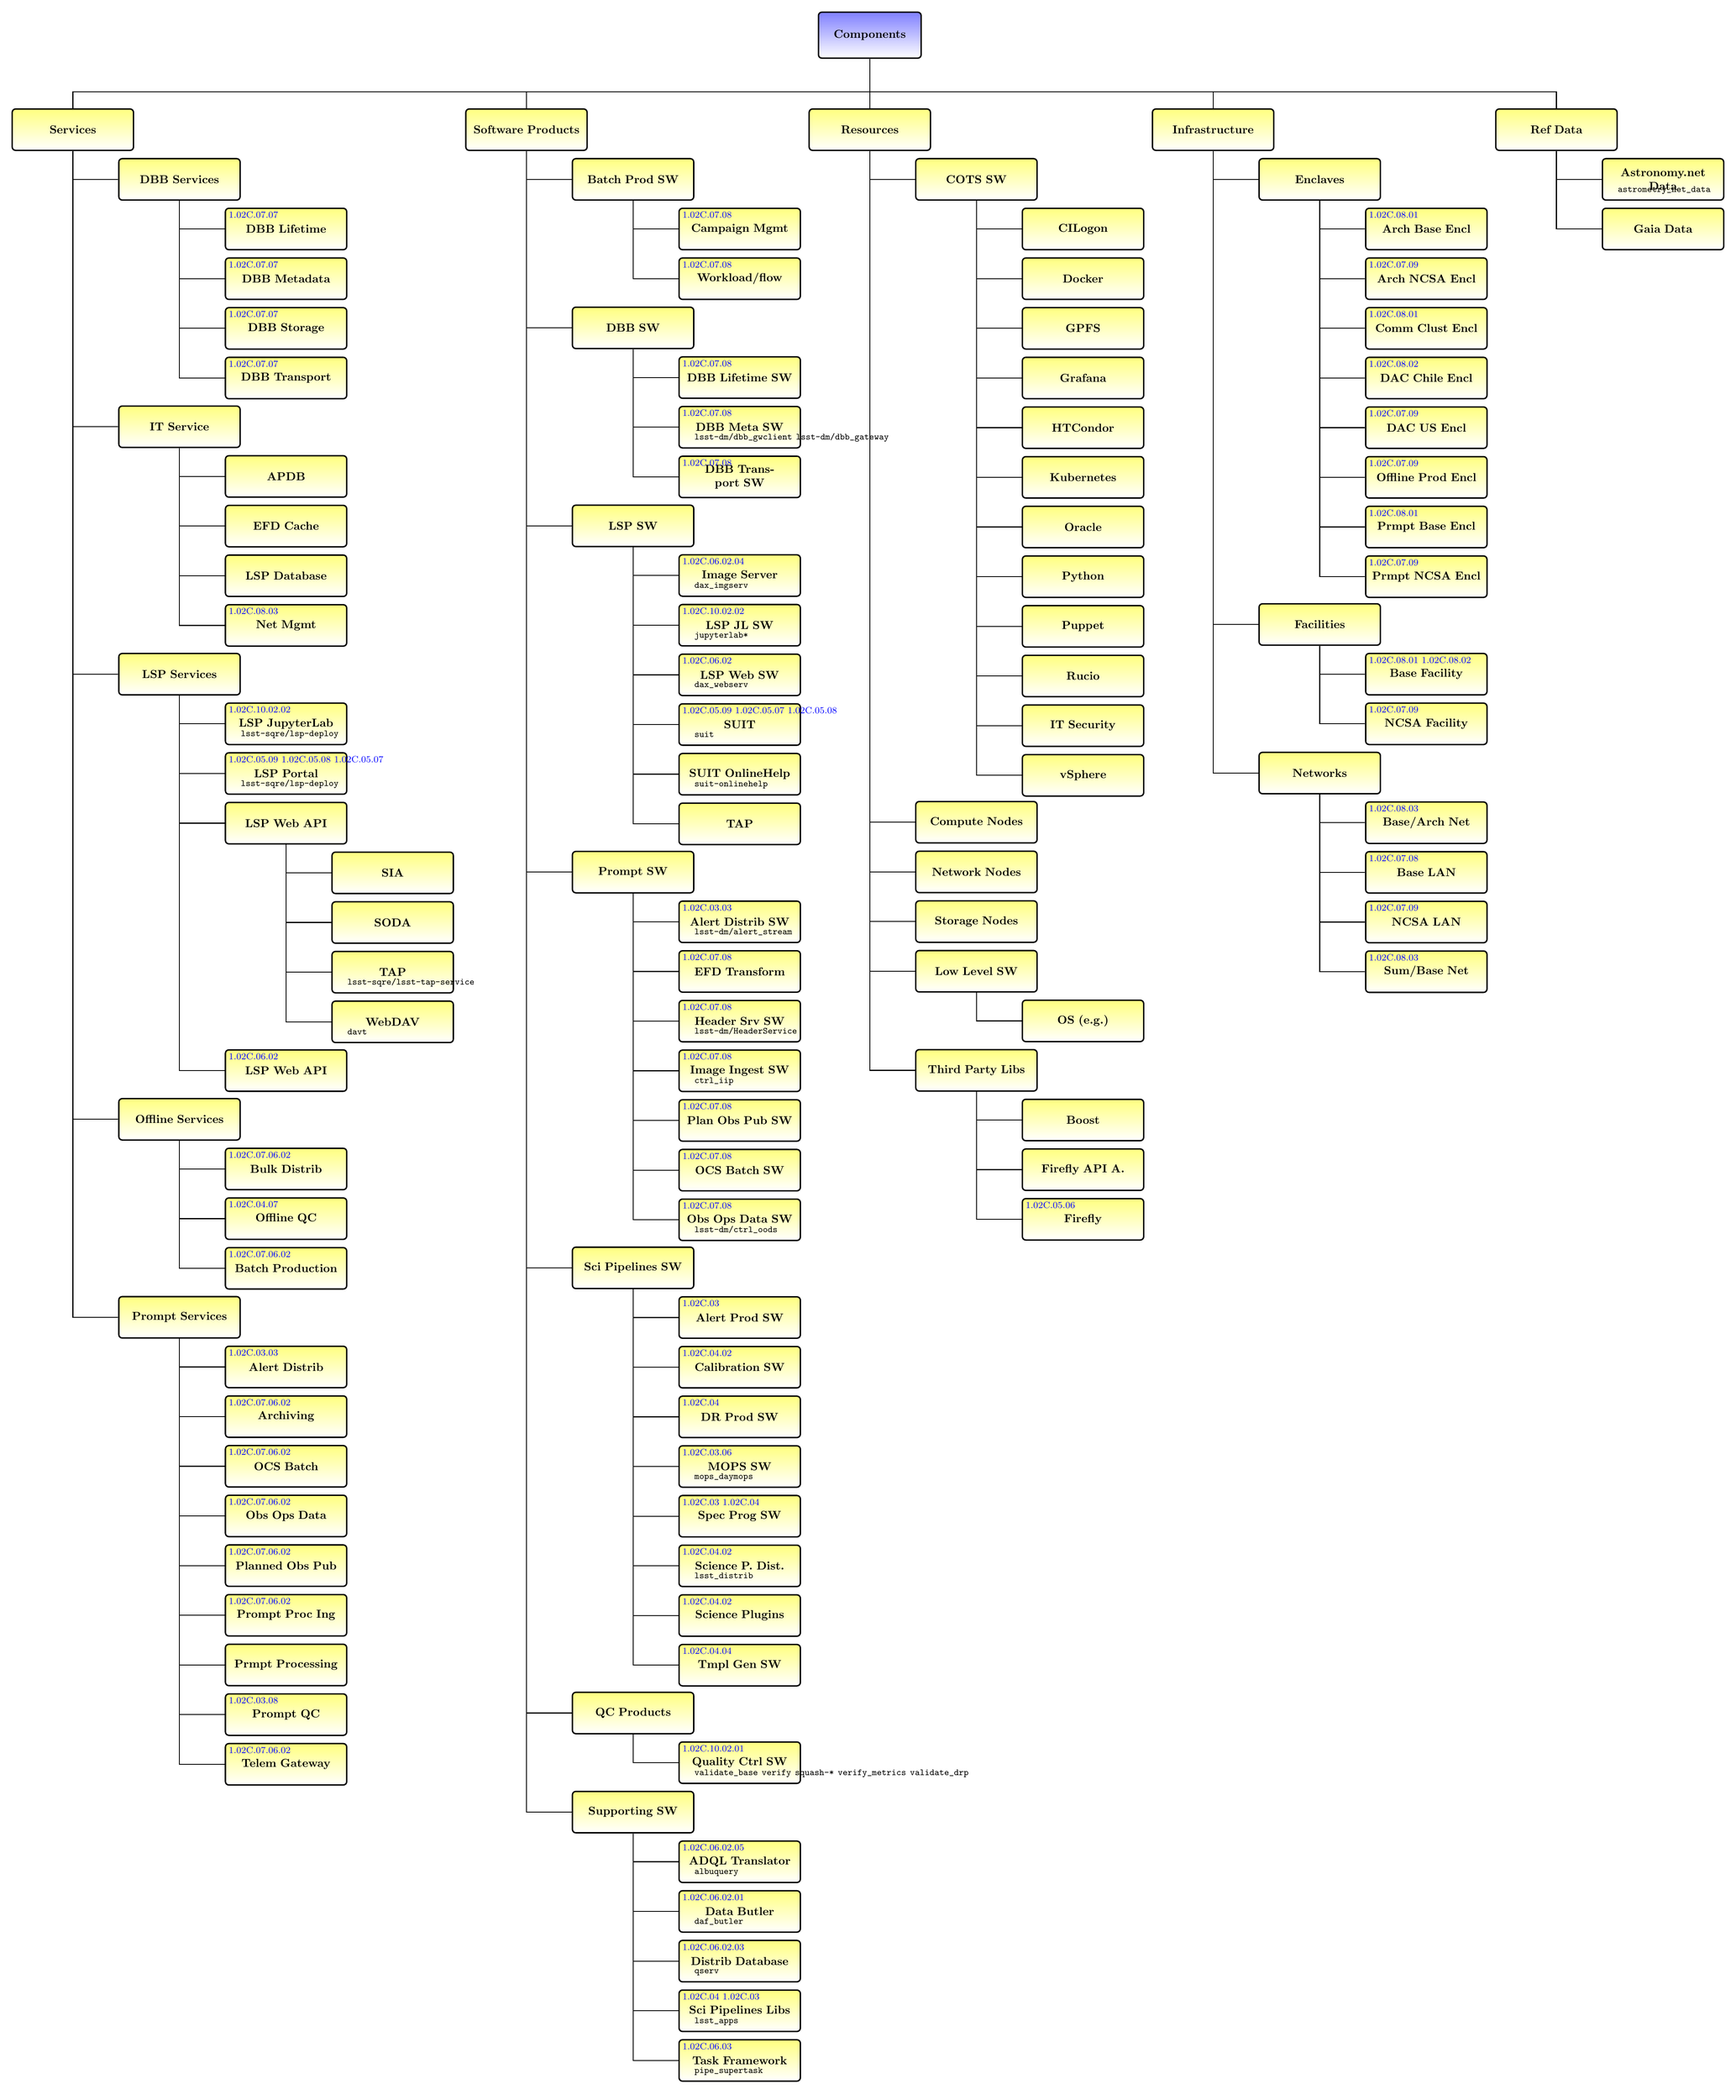
\begin{tikzpicture}[node distance=0mm]


\node (DMSRV) [pbox, 
] {\textbf{Services
} };\node [below right] at (DMSRV.north west) {\footnotesize \color{blue}} ;

\node (DBBSRV) [pbox,below right=6pt and -14pt of DMSRV] {\textbf{DBB Services
} };\node [below right] at (DBBSRV.north west) {\footnotesize \color{blue}} ;

 \draw[pline] (DMSRV.south) -| ++(0,0) |- (DBBSRV.west); 
\node (DBBLIFESRV) [pbox,below right=6pt and -14pt of DBBSRV] {\textbf{DBB Lifetime
} };\node [below right] at (DBBLIFESRV.north west) {\footnotesize \color{blue}1.02C.07.07} ;

 \draw[pline] (DBBSRV.south) -| ++(0,0) |- (DBBLIFESRV.west); 
\node (DBBMDSRV) [pbox,below=6pt of DBBLIFESRV] {\textbf{DBB Metadata
} };\node [below right] at (DBBMDSRV.north west) {\footnotesize \color{blue}1.02C.07.07} ;

 \draw[pline] (DBBSRV.south) -| ++(0,0) |- (DBBMDSRV.west); 
\node (DBBSTRSRV) [pbox,below=6pt of DBBMDSRV] {\textbf{DBB Storage
} };\node [below right] at (DBBSTRSRV.north west) {\footnotesize \color{blue}1.02C.07.07} ;

 \draw[pline] (DBBSRV.south) -| ++(0,0) |- (DBBSTRSRV.west); 
\node (DBBTRSRV) [pbox,below=6pt of DBBSTRSRV] {\textbf{DBB Transport
} };\node [below right] at (DBBTRSRV.north west) {\footnotesize \color{blue}1.02C.07.07} ;

 \draw[pline] (DBBSRV.south) -| ++(0,0) |- (DBBTRSRV.west); 
\node (ITSRV) [pbox,below=178pt of DBBSRV] {\textbf{IT Service
} };\node [below right] at (ITSRV.north west) {\footnotesize \color{blue}} ;

 \draw[pline] (DMSRV.south) -| ++(0,0) |- (ITSRV.west); 
\node (APDB) [pbox,below right=6pt and -14pt of ITSRV] {\textbf{APDB
} };\node [below right] at (APDB.north west) {\footnotesize \color{blue}} ;

 \draw[pline] (ITSRV.south) -| ++(0,0) |- (APDB.west); 
\node (EFDB) [pbox,below=6pt of APDB] {\textbf{EFD Cache
} };\node [below right] at (EFDB.north west) {\footnotesize \color{blue}} ;

 \draw[pline] (ITSRV.south) -| ++(0,0) |- (EFDB.west); 
\node (LSPDB) [pbox,below=6pt of EFDB] {\textbf{LSP Database
} };\node [below right] at (LSPDB.north west) {\footnotesize \color{blue}} ;

 \draw[pline] (ITSRV.south) -| ++(0,0) |- (LSPDB.west); 
\node (NETMGMT) [pbox,below=6pt of LSPDB] {\textbf{Net Mgmt
} };\node [below right] at (NETMGMT.north west) {\footnotesize \color{blue}1.02C.08.03} ;

 \draw[pline] (ITSRV.south) -| ++(0,0) |- (NETMGMT.west); 
\node (LSPSRV) [pbox,below=178pt of ITSRV] {\textbf{LSP Services
} };\node [below right] at (LSPSRV.north west) {\footnotesize \color{blue}} ;

 \draw[pline] (DMSRV.south) -| ++(0,0) |- (LSPSRV.west); 
\node (LSPJLSRV) [pbox,below right=6pt and -14pt of LSPSRV] {\textbf{LSP JupyterLab
} };\node [below right] at (LSPJLSRV.north west) {\footnotesize \color{blue}1.02C.10.02.02} ;
\node (LSPJLSRVpkg) [tbox,below=3mm of LSPJLSRV.north] {{\footnotesize \color{black} \begin{verbatim} lsst-sqre/lsp-deploy \end{verbatim} }  };

 \draw[pline] (LSPSRV.south) -| ++(0,0) |- (LSPJLSRV.west); 
\node (LSPPRTLSRV) [pbox,below=6pt of LSPJLSRV] {\textbf{LSP Portal
} };\node [below right] at (LSPPRTLSRV.north west) {\footnotesize \color{blue}1.02C.05.09 1.02C.05.08 1.02C.05.07} ;
\node (LSPPRTLSRVpkg) [tbox,below=3mm of LSPPRTLSRV.north] {{\footnotesize \color{black} \begin{verbatim} lsst-sqre/lsp-deploy \end{verbatim} }  };

 \draw[pline] (LSPSRV.south) -| ++(0,0) |- (LSPPRTLSRV.west); 
\node (LSPWAPI) [pbox,below=6pt of LSPPRTLSRV] {\textbf{LSP Web API
} };\node [below right] at (LSPWAPI.north west) {\footnotesize \color{blue}} ;

 \draw[pline] (LSPSRV.south) -| ++(0,0) |- (LSPWAPI.west); 
\node (SIASRV) [pbox,below right=6pt and -14pt of LSPWAPI] {\textbf{SIA
} };\node [below right] at (SIASRV.north west) {\footnotesize \color{blue}} ;

 \draw[pline] (LSPWAPI.south) -| ++(0,0) |- (SIASRV.west); 
\node (SODA) [pbox,below=6pt of SIASRV] {\textbf{SODA
} };\node [below right] at (SODA.north west) {\footnotesize \color{blue}} ;

 \draw[pline] (LSPWAPI.south) -| ++(0,0) |- (SODA.west); 
\node (TAPSEV) [pbox,below=6pt of SODA] {\textbf{TAP
} };\node [below right] at (TAPSEV.north west) {\footnotesize \color{blue}} ;
\node (TAPSEVpkg) [tbox,below=3mm of TAPSEV.north] {{\footnotesize \color{black} \begin{verbatim} lsst-sqre/lsst-tap-service \end{verbatim} }  };

 \draw[pline] (LSPWAPI.south) -| ++(0,0) |- (TAPSEV.west); 
\node (WDAV) [pbox,below=6pt of TAPSEV] {\textbf{WebDAV
} };\node [below right] at (WDAV.north west) {\footnotesize \color{blue}} ;
\node (WDAVpkg) [tbox,below=3mm of WDAV.north] {{\footnotesize \color{black} \begin{verbatim} davt \end{verbatim} }  };

 \draw[pline] (LSPWAPI.south) -| ++(0,0) |- (WDAV.west); 
\node (LSPWEBSRV) [pbox,below=178pt of LSPWAPI] {\textbf{LSP Web API
} };\node [below right] at (LSPWEBSRV.north west) {\footnotesize \color{blue}1.02C.06.02} ;

 \draw[pline] (LSPSRV.south) -| ++(0,0) |- (LSPWEBSRV.west); 
\node (OFFLSRV) [pbox,below=350pt of LSPSRV] {\textbf{Offline Services
} };\node [below right] at (OFFLSRV.north west) {\footnotesize \color{blue}} ;

 \draw[pline] (DMSRV.south) -| ++(0,0) |- (OFFLSRV.west); 
\node (BULKDSRV) [pbox,below right=6pt and -14pt of OFFLSRV] {\textbf{Bulk Distrib
} };\node [below right] at (BULKDSRV.north west) {\footnotesize \color{blue}1.02C.07.06.02} ;

 \draw[pline] (OFFLSRV.south) -| ++(0,0) |- (BULKDSRV.west); 
\node (OFFLQCSRV) [pbox,below=6pt of BULKDSRV] {\textbf{Offline QC
} };\node [below right] at (OFFLQCSRV.north west) {\footnotesize \color{blue}1.02C.04.07} ;

 \draw[pline] (OFFLSRV.south) -| ++(0,0) |- (OFFLQCSRV.west); 
\node (PRODSRV) [pbox,below=6pt of OFFLQCSRV] {\textbf{Batch Production
} };\node [below right] at (PRODSRV.north west) {\footnotesize \color{blue}1.02C.07.06.02} ;

 \draw[pline] (OFFLSRV.south) -| ++(0,0) |- (PRODSRV.west); 
\node (PRSRV) [pbox,below=135pt of OFFLSRV] {\textbf{Prompt Services
} };\node [below right] at (PRSRV.north west) {\footnotesize \color{blue}} ;

 \draw[pline] (DMSRV.south) -| ++(0,0) |- (PRSRV.west); 
\node (ALRTDSTSRV) [pbox,below right=6pt and -14pt of PRSRV] {\textbf{Alert Distrib
} };\node [below right] at (ALRTDSTSRV.north west) {\footnotesize \color{blue}1.02C.03.03} ;

 \draw[pline] (PRSRV.south) -| ++(0,0) |- (ALRTDSTSRV.west); 
\node (ARCSRV) [pbox,below=6pt of ALRTDSTSRV] {\textbf{Archiving
} };\node [below right] at (ARCSRV.north west) {\footnotesize \color{blue}1.02C.07.06.02} ;

 \draw[pline] (PRSRV.south) -| ++(0,0) |- (ARCSRV.west); 
\node (OCSBATSRV) [pbox,below=6pt of ARCSRV] {\textbf{OCS Batch
} };\node [below right] at (OCSBATSRV.north west) {\footnotesize \color{blue}1.02C.07.06.02} ;

 \draw[pline] (PRSRV.south) -| ++(0,0) |- (OCSBATSRV.west); 
\node (OODSSRV) [pbox,below=6pt of OCSBATSRV] {\textbf{Obs Ops Data
} };\node [below right] at (OODSSRV.north west) {\footnotesize \color{blue}1.02C.07.06.02} ;

 \draw[pline] (PRSRV.south) -| ++(0,0) |- (OODSSRV.west); 
\node (POPSRV) [pbox,below=6pt of OODSSRV] {\textbf{Planned Obs Pub
} };\node [below right] at (POPSRV.north west) {\footnotesize \color{blue}1.02C.07.06.02} ;

 \draw[pline] (PRSRV.south) -| ++(0,0) |- (POPSRV.west); 
\node (PRPINGSRV) [pbox,below=6pt of POPSRV] {\textbf{Prompt Proc Ing
} };\node [below right] at (PRPINGSRV.north west) {\footnotesize \color{blue}1.02C.07.06.02} ;

 \draw[pline] (PRSRV.south) -| ++(0,0) |- (PRPINGSRV.west); 
\node (PRPRSRV) [pbox,below=6pt of PRPINGSRV] {\textbf{Prmpt Processing
} };\node [below right] at (PRPRSRV.north west) {\footnotesize \color{blue}} ;

 \draw[pline] (PRSRV.south) -| ++(0,0) |- (PRPRSRV.west); 
\node (PRQCSRV) [pbox,below=6pt of PRPRSRV] {\textbf{Prompt QC
} };\node [below right] at (PRQCSRV.north west) {\footnotesize \color{blue}1.02C.03.08} ;

 \draw[pline] (PRSRV.south) -| ++(0,0) |- (PRQCSRV.west); 
\node (TMGSRV) [pbox,below=6pt of PRQCSRV] {\textbf{Telem Gateway
} };\node [below right] at (TMGSRV.north west) {\footnotesize \color{blue}1.02C.07.06.02} ;

 \draw[pline] (PRSRV.south) -| ++(0,0) |- (TMGSRV.west); 
\node (DMSW) [pbox, 
right=288pt of DMSRV] {\textbf{Software Products
} };\node [below right] at (DMSW.north west) {\footnotesize \color{blue}} ;

\node (BPP) [pbox,below right=6pt and -14pt of DMSW] {\textbf{Batch Prod SW
} };\node [below right] at (BPP.north west) {\footnotesize \color{blue}} ;

 \draw[pline] (DMSW.south) -| ++(0,0) |- (BPP.west); 
\node (CMPGN) [pbox,below right=6pt and -14pt of BPP] {\textbf{Campaign Mgmt
} };\node [below right] at (CMPGN.north west) {\footnotesize \color{blue}1.02C.07.08} ;

 \draw[pline] (BPP.south) -| ++(0,0) |- (CMPGN.west); 
\node (WLWF) [pbox,below=6pt of CMPGN] {\textbf{Workload/flow
} };\node [below right] at (WLWF.north west) {\footnotesize \color{blue}1.02C.07.08} ;

 \draw[pline] (BPP.south) -| ++(0,0) |- (WLWF.west); 
\node (DBB) [pbox,below=92pt of BPP] {\textbf{DBB SW
} };\node [below right] at (DBB.north west) {\footnotesize \color{blue}} ;

 \draw[pline] (DMSW.south) -| ++(0,0) |- (DBB.west); 
\node (DBBLIFE) [pbox,below right=6pt and -14pt of DBB] {\textbf{DBB Lifetime SW
} };\node [below right] at (DBBLIFE.north west) {\footnotesize \color{blue}1.02C.07.08} ;

 \draw[pline] (DBB.south) -| ++(0,0) |- (DBBLIFE.west); 
\node (DBBMD) [pbox,below=6pt of DBBLIFE] {\textbf{DBB Meta SW
} };\node [below right] at (DBBMD.north west) {\footnotesize \color{blue}1.02C.07.08} ;
\node (DBBMDpkg) [tbox,below=3mm of DBBMD.north] {{\footnotesize \color{black} \begin{verbatim} lsst-dm/dbb_gwclient lsst-dm/dbb_gateway \end{verbatim} }  };

 \draw[pline] (DBB.south) -| ++(0,0) |- (DBBMD.west); 
\node (DBBTR) [pbox,below=6pt of DBBMD] {\textbf{DBB Transport SW
} };\node [below right] at (DBBTR.north west) {\footnotesize \color{blue}1.02C.07.08} ;

 \draw[pline] (DBB.south) -| ++(0,0) |- (DBBTR.west); 
\node (LSP) [pbox,below=135pt of DBB] {\textbf{LSP SW
} };\node [below right] at (LSP.north west) {\footnotesize \color{blue}} ;

 \draw[pline] (DMSW.south) -| ++(0,0) |- (LSP.west); 
\node (DAXIMG) [pbox,below right=6pt and -14pt of LSP] {\textbf{Image Server
} };\node [below right] at (DAXIMG.north west) {\footnotesize \color{blue}1.02C.06.02.04} ;
\node (DAXIMGpkg) [tbox,below=3mm of DAXIMG.north] {{\footnotesize \color{black} \begin{verbatim} dax_imgserv \end{verbatim} }  };

 \draw[pline] (LSP.south) -| ++(0,0) |- (DAXIMG.west); 
\node (LSPJL) [pbox,below=6pt of DAXIMG] {\textbf{LSP JL SW
} };\node [below right] at (LSPJL.north west) {\footnotesize \color{blue}1.02C.10.02.02} ;
\node (LSPJLpkg) [tbox,below=3mm of LSPJL.north] {{\footnotesize \color{black} \begin{verbatim} jupyterlab* \end{verbatim} }  };

 \draw[pline] (LSP.south) -| ++(0,0) |- (LSPJL.west); 
\node (LSPWEB) [pbox,below=6pt of LSPJL] {\textbf{LSP Web SW
} };\node [below right] at (LSPWEB.north west) {\footnotesize \color{blue}1.02C.06.02} ;
\node (LSPWEBpkg) [tbox,below=3mm of LSPWEB.north] {{\footnotesize \color{black} \begin{verbatim} dax_webserv \end{verbatim} }  };

 \draw[pline] (LSP.south) -| ++(0,0) |- (LSPWEB.west); 
\node (SUIT) [pbox,below=6pt of LSPWEB] {\textbf{SUIT
} };\node [below right] at (SUIT.north west) {\footnotesize \color{blue}1.02C.05.09 1.02C.05.07 1.02C.05.08} ;
\node (SUITpkg) [tbox,below=3mm of SUIT.north] {{\footnotesize \color{black} \begin{verbatim} suit \end{verbatim} }  };

 \draw[pline] (LSP.south) -| ++(0,0) |- (SUIT.west); 
\node (SUITOH) [pbox,below=6pt of SUIT] {\textbf{SUIT OnlineHelp
} };\node [below right] at (SUITOH.north west) {\footnotesize \color{blue}} ;
\node (SUITOHpkg) [tbox,below=3mm of SUITOH.north] {{\footnotesize \color{black} \begin{verbatim} suit-onlinehelp \end{verbatim} }  };

 \draw[pline] (LSP.south) -| ++(0,0) |- (SUITOH.west); 
\node (TAPSW) [pbox,below=6pt of SUITOH] {\textbf{TAP
} };\node [below right] at (TAPSW.north west) {\footnotesize \color{blue}} ;

 \draw[pline] (LSP.south) -| ++(0,0) |- (TAPSW.west); 
\node (PR) [pbox,below=264pt of LSP] {\textbf{Prompt SW
} };\node [below right] at (PR.north west) {\footnotesize \color{blue}} ;

 \draw[pline] (DMSW.south) -| ++(0,0) |- (PR.west); 
\node (ALRTDSTR) [pbox,below right=6pt and -14pt of PR] {\textbf{Alert Distrib SW
} };\node [below right] at (ALRTDSTR.north west) {\footnotesize \color{blue}1.02C.03.03} ;
\node (ALRTDSTRpkg) [tbox,below=3mm of ALRTDSTR.north] {{\footnotesize \color{black} \begin{verbatim} lsst-dm/alert_stream \end{verbatim} }  };

 \draw[pline] (PR.south) -| ++(0,0) |- (ALRTDSTR.west); 
\node (EFDT) [pbox,below=6pt of ALRTDSTR] {\textbf{EFD Transform
} };\node [below right] at (EFDT.north west) {\footnotesize \color{blue}1.02C.07.08} ;

 \draw[pline] (PR.south) -| ++(0,0) |- (EFDT.west); 
\node (HEADER) [pbox,below=6pt of EFDT] {\textbf{Header Srv SW
} };\node [below right] at (HEADER.north west) {\footnotesize \color{blue}1.02C.07.08} ;
\node (HEADERpkg) [tbox,below=3mm of HEADER.north] {{\footnotesize \color{black} \begin{verbatim} lsst-dm/HeaderService \end{verbatim} }  };

 \draw[pline] (PR.south) -| ++(0,0) |- (HEADER.west); 
\node (IIP) [pbox,below=6pt of HEADER] {\textbf{Image Ingest SW
} };\node [below right] at (IIP.north west) {\footnotesize \color{blue}1.02C.07.08} ;
\node (IIPpkg) [tbox,below=3mm of IIP.north] {{\footnotesize \color{black} \begin{verbatim} ctrl_iip \end{verbatim} }  };

 \draw[pline] (PR.south) -| ++(0,0) |- (IIP.west); 
\node (OBSPUB) [pbox,below=6pt of IIP] {\textbf{Plan Obs Pub SW
} };\node [below right] at (OBSPUB.north west) {\footnotesize \color{blue}1.02C.07.08} ;

 \draw[pline] (PR.south) -| ++(0,0) |- (OBSPUB.west); 
\node (OCSBAT) [pbox,below=6pt of OBSPUB] {\textbf{OCS Batch SW
} };\node [below right] at (OCSBAT.north west) {\footnotesize \color{blue}1.02C.07.08} ;

 \draw[pline] (PR.south) -| ++(0,0) |- (OCSBAT.west); 
\node (OODS) [pbox,below=6pt of OCSBAT] {\textbf{Obs Ops Data SW
} };\node [below right] at (OODS.north west) {\footnotesize \color{blue}1.02C.07.08} ;
\node (OODSpkg) [tbox,below=3mm of OODS.north] {{\footnotesize \color{black} \begin{verbatim} lsst-dm/ctrl_oods \end{verbatim} }  };

 \draw[pline] (PR.south) -| ++(0,0) |- (OODS.west); 
\node (PRODN) [pbox,below=307pt of PR] {\textbf{Sci Pipelines SW
} };\node [below right] at (PRODN.north west) {\footnotesize \color{blue}} ;

 \draw[pline] (DMSW.south) -| ++(0,0) |- (PRODN.west); 
\node (APPRMPT) [pbox,below right=6pt and -14pt of PRODN] {\textbf{Alert Prod SW
} };\node [below right] at (APPRMPT.north west) {\footnotesize \color{blue}1.02C.03} ;

 \draw[pline] (PRODN.south) -| ++(0,0) |- (APPRMPT.west); 
\node (DMCAL) [pbox,below=6pt of APPRMPT] {\textbf{Calibration SW
} };\node [below right] at (DMCAL.north west) {\footnotesize \color{blue}1.02C.04.02} ;

 \draw[pline] (PRODN.south) -| ++(0,0) |- (DMCAL.west); 
\node (DRP) [pbox,below=6pt of DMCAL] {\textbf{DR Prod SW
} };\node [below right] at (DRP.north west) {\footnotesize \color{blue}1.02C.04} ;

 \draw[pline] (PRODN.south) -| ++(0,0) |- (DRP.west); 
\node (MOPS) [pbox,below=6pt of DRP] {\textbf{MOPS SW
} };\node [below right] at (MOPS.north west) {\footnotesize \color{blue}1.02C.03.06} ;
\node (MOPSpkg) [tbox,below=3mm of MOPS.north] {{\footnotesize \color{black} \begin{verbatim} mops_daymops \end{verbatim} }  };

 \draw[pline] (PRODN.south) -| ++(0,0) |- (MOPS.west); 
\node (SP) [pbox,below=6pt of MOPS] {\textbf{Spec Prog SW
} };\node [below right] at (SP.north west) {\footnotesize \color{blue}1.02C.03 1.02C.04} ;

 \draw[pline] (PRODN.south) -| ++(0,0) |- (SP.west); 
\node (SPDIST) [pbox,below=6pt of SP] {\textbf{Science P. Dist.
} };\node [below right] at (SPDIST.north west) {\footnotesize \color{blue}1.02C.04.02} ;
\node (SPDISTpkg) [tbox,below=3mm of SPDIST.north] {{\footnotesize \color{black} \begin{verbatim} lsst_distrib \end{verbatim} }  };

 \draw[pline] (PRODN.south) -| ++(0,0) |- (SPDIST.west); 
\node (SPLUG) [pbox,below=6pt of SPDIST] {\textbf{Science Plugins
} };\node [below right] at (SPLUG.north west) {\footnotesize \color{blue}1.02C.04.02} ;

 \draw[pline] (PRODN.south) -| ++(0,0) |- (SPLUG.west); 
\node (TMPLGEN) [pbox,below=6pt of SPLUG] {\textbf{Tmpl Gen SW
} };\node [below right] at (TMPLGEN.north west) {\footnotesize \color{blue}1.02C.04.04} ;

 \draw[pline] (PRODN.south) -| ++(0,0) |- (TMPLGEN.west); 
\node (QC) [pbox,below=350pt of PRODN] {\textbf{QC Products
} };\node [below right] at (QC.north west) {\footnotesize \color{blue}} ;

 \draw[pline] (DMSW.south) -| ++(0,0) |- (QC.west); 
\node (QCSW) [pbox,below right=6pt and -14pt of QC] {\textbf{Quality Ctrl SW
} };\node [below right] at (QCSW.north west) {\footnotesize \color{blue}1.02C.10.02.01} ;
\node (QCSWpkg) [tbox,below=3mm of QCSW.north] {{\footnotesize \color{black} \begin{verbatim} validate_base verify squash-* verify_metrics validate_drp \end{verbatim} }  };

 \draw[pline] (QC.south) -| ++(0,0) |- (QCSW.west); 
\node (SUPPSW) [pbox,below=49pt of QC] {\textbf{Supporting SW
} };\node [below right] at (SUPPSW.north west) {\footnotesize \color{blue}} ;

 \draw[pline] (DMSW.south) -| ++(0,0) |- (SUPPSW.west); 
\node (ADQL) [pbox,below right=6pt and -14pt of SUPPSW] {\textbf{ADQL Translator
} };\node [below right] at (ADQL.north west) {\footnotesize \color{blue}1.02C.06.02.05} ;
\node (ADQLpkg) [tbox,below=3mm of ADQL.north] {{\footnotesize \color{black} \begin{verbatim} albuquery \end{verbatim} }  };

 \draw[pline] (SUPPSW.south) -| ++(0,0) |- (ADQL.west); 
\node (BUTLER) [pbox,below=6pt of ADQL] {\textbf{Data Butler
} };\node [below right] at (BUTLER.north west) {\footnotesize \color{blue}1.02C.06.02.01} ;
\node (BUTLERpkg) [tbox,below=3mm of BUTLER.north] {{\footnotesize \color{black} \begin{verbatim} daf_butler \end{verbatim} }  };

 \draw[pline] (SUPPSW.south) -| ++(0,0) |- (BUTLER.west); 
\node (QSERV) [pbox,below=6pt of BUTLER] {\textbf{Distrib Database
} };\node [below right] at (QSERV.north west) {\footnotesize \color{blue}1.02C.06.02.03} ;
\node (QSERVpkg) [tbox,below=3mm of QSERV.north] {{\footnotesize \color{black} \begin{verbatim} qserv \end{verbatim} }  };

 \draw[pline] (SUPPSW.south) -| ++(0,0) |- (QSERV.west); 
\node (SCIPIPE) [pbox,below=6pt of QSERV] {\textbf{Sci Pipelines Libs
} };\node [below right] at (SCIPIPE.north west) {\footnotesize \color{blue}1.02C.04 1.02C.03} ;
\node (SCIPIPEpkg) [tbox,below=3mm of SCIPIPE.north] {{\footnotesize \color{black} \begin{verbatim} lsst_apps \end{verbatim} }  };

 \draw[pline] (SUPPSW.south) -| ++(0,0) |- (SCIPIPE.west); 
\node (TXF) [pbox,below=6pt of SCIPIPE] {\textbf{Task Framework
} };\node [below right] at (TXF.north west) {\footnotesize \color{blue}1.02C.06.03} ;
\node (TXFpkg) [tbox,below=3mm of TXF.north] {{\footnotesize \color{black} \begin{verbatim} pipe_supertask \end{verbatim} }  };

 \draw[pline] (SUPPSW.south) -| ++(0,0) |- (TXF.west); 
\node (HWCOTS) [pbox, 
right=192pt of DMSW] {\textbf{Resources
} };\node [below right] at (HWCOTS.north west) {\footnotesize \color{blue}} ;

\node (COTS) [pbox,below right=6pt and -14pt of HWCOTS] {\textbf{COTS SW
} };\node [below right] at (COTS.north west) {\footnotesize \color{blue}} ;

 \draw[pline] (HWCOTS.south) -| ++(0,0) |- (COTS.west); 
\node (CILOGON) [pbox,below right=6pt and -14pt of COTS] {\textbf{CILogon
} };\node [below right] at (CILOGON.north west) {\footnotesize \color{blue}} ;

 \draw[pline] (COTS.south) -| ++(0,0) |- (CILOGON.west); 
\node (DOCKER) [pbox,below=6pt of CILOGON] {\textbf{Docker
} };\node [below right] at (DOCKER.north west) {\footnotesize \color{blue}} ;

 \draw[pline] (COTS.south) -| ++(0,0) |- (DOCKER.west); 
\node (GPFS) [pbox,below=6pt of DOCKER] {\textbf{GPFS
} };\node [below right] at (GPFS.north west) {\footnotesize \color{blue}} ;

 \draw[pline] (COTS.south) -| ++(0,0) |- (GPFS.west); 
\node (GRAFANA) [pbox,below=6pt of GPFS] {\textbf{Grafana
} };\node [below right] at (GRAFANA.north west) {\footnotesize \color{blue}} ;

 \draw[pline] (COTS.south) -| ++(0,0) |- (GRAFANA.west); 
\node (HTCONDOR) [pbox,below=6pt of GRAFANA] {\textbf{HTCondor
} };\node [below right] at (HTCONDOR.north west) {\footnotesize \color{blue}} ;

 \draw[pline] (COTS.south) -| ++(0,0) |- (HTCONDOR.west); 
\node (K8S) [pbox,below=6pt of HTCONDOR] {\textbf{Kubernetes
} };\node [below right] at (K8S.north west) {\footnotesize \color{blue}} ;

 \draw[pline] (COTS.south) -| ++(0,0) |- (K8S.west); 
\node (ORACLE) [pbox,below=6pt of K8S] {\textbf{Oracle
} };\node [below right] at (ORACLE.north west) {\footnotesize \color{blue}} ;

 \draw[pline] (COTS.south) -| ++(0,0) |- (ORACLE.west); 
\node (PTH) [pbox,below=6pt of ORACLE] {\textbf{Python
} };\node [below right] at (PTH.north west) {\footnotesize \color{blue}} ;

 \draw[pline] (COTS.south) -| ++(0,0) |- (PTH.west); 
\node (PUPPET) [pbox,below=6pt of PTH] {\textbf{Puppet
} };\node [below right] at (PUPPET.north west) {\footnotesize \color{blue}} ;

 \draw[pline] (COTS.south) -| ++(0,0) |- (PUPPET.west); 
\node (RUCIO) [pbox,below=6pt of PUPPET] {\textbf{Rucio
} };\node [below right] at (RUCIO.north west) {\footnotesize \color{blue}} ;

 \draw[pline] (COTS.south) -| ++(0,0) |- (RUCIO.west); 
\node (SECURITY) [pbox,below=6pt of RUCIO] {\textbf{IT Security
} };\node [below right] at (SECURITY.north west) {\footnotesize \color{blue}} ;

 \draw[pline] (COTS.south) -| ++(0,0) |- (SECURITY.west); 
\node (VSPHERE) [pbox,below=6pt of SECURITY] {\textbf{vSphere
} };\node [below right] at (VSPHERE.north west) {\footnotesize \color{blue}} ;

 \draw[pline] (COTS.south) -| ++(0,0) |- (VSPHERE.west); 
\node (HWCOMP) [pbox,below=522pt of COTS] {\textbf{Compute Nodes
} };\node [below right] at (HWCOMP.north west) {\footnotesize \color{blue}} ;

 \draw[pline] (HWCOTS.south) -| ++(0,0) |- (HWCOMP.west); 
\node (HWNET) [pbox,below=6pt of HWCOMP] {\textbf{Network Nodes
} };\node [below right] at (HWNET.north west) {\footnotesize \color{blue}} ;

 \draw[pline] (HWCOTS.south) -| ++(0,0) |- (HWNET.west); 
\node (HWSTOR) [pbox,below=6pt of HWNET] {\textbf{Storage Nodes
} };\node [below right] at (HWSTOR.north west) {\footnotesize \color{blue}} ;

 \draw[pline] (HWCOTS.south) -| ++(0,0) |- (HWSTOR.west); 
\node (LLSW) [pbox,below=6pt of HWSTOR] {\textbf{Low Level SW
} };\node [below right] at (LLSW.north west) {\footnotesize \color{blue}} ;

 \draw[pline] (HWCOTS.south) -| ++(0,0) |- (LLSW.west); 
\node (CENTOS) [pbox,below right=6pt and -14pt of LLSW] {\textbf{OS (e.g.)
} };\node [below right] at (CENTOS.north west) {\footnotesize \color{blue}} ;

 \draw[pline] (LLSW.south) -| ++(0,0) |- (CENTOS.west); 
\node (THPL) [pbox,below=49pt of LLSW] {\textbf{Third Party Libs
} };\node [below right] at (THPL.north west) {\footnotesize \color{blue}} ;

 \draw[pline] (HWCOTS.south) -| ++(0,0) |- (THPL.west); 
\node (BOOST) [pbox,below right=6pt and -14pt of THPL] {\textbf{Boost
} };\node [below right] at (BOOST.north west) {\footnotesize \color{blue}} ;

 \draw[pline] (THPL.south) -| ++(0,0) |- (BOOST.west); 
\node (FFAA) [pbox,below=6pt of BOOST] {\textbf{Firefly API A.
} };\node [below right] at (FFAA.north west) {\footnotesize \color{blue}} ;

 \draw[pline] (THPL.south) -| ++(0,0) |- (FFAA.west); 
\node (FIREFLY) [pbox,below=6pt of FFAA] {\textbf{Firefly
} };\node [below right] at (FIREFLY.north west) {\footnotesize \color{blue}1.02C.05.06} ;

 \draw[pline] (THPL.south) -| ++(0,0) |- (FIREFLY.west); 
\node (INFRA) [pbox, 
right=192pt of HWCOTS] {\textbf{Infrastructure
} };\node [below right] at (INFRA.north west) {\footnotesize \color{blue}} ;

\node (ENC) [pbox,below right=6pt and -14pt of INFRA] {\textbf{Enclaves
} };\node [below right] at (ENC.north west) {\footnotesize \color{blue}} ;

 \draw[pline] (INFRA.south) -| ++(0,0) |- (ENC.west); 
\node (ENCARCB) [pbox,below right=6pt and -14pt of ENC] {\textbf{Arch Base Encl
} };\node [below right] at (ENCARCB.north west) {\footnotesize \color{blue}1.02C.08.01} ;

 \draw[pline] (ENC.south) -| ++(0,0) |- (ENCARCB.west); 
\node (ENCARCN) [pbox,below=6pt of ENCARCB] {\textbf{Arch NCSA Encl
} };\node [below right] at (ENCARCN.north west) {\footnotesize \color{blue}1.02C.07.09} ;

 \draw[pline] (ENC.south) -| ++(0,0) |- (ENCARCN.west); 
\node (ENCCOMM) [pbox,below=6pt of ENCARCN] {\textbf{Comm Clust Encl
} };\node [below right] at (ENCCOMM.north west) {\footnotesize \color{blue}1.02C.08.01} ;

 \draw[pline] (ENC.south) -| ++(0,0) |- (ENCCOMM.west); 
\node (ENCDACC) [pbox,below=6pt of ENCCOMM] {\textbf{DAC Chile Encl
} };\node [below right] at (ENCDACC.north west) {\footnotesize \color{blue}1.02C.08.02} ;

 \draw[pline] (ENC.south) -| ++(0,0) |- (ENCDACC.west); 
\node (ENCDACU) [pbox,below=6pt of ENCDACC] {\textbf{DAC US Encl
} };\node [below right] at (ENCDACU.north west) {\footnotesize \color{blue}1.02C.07.09} ;

 \draw[pline] (ENC.south) -| ++(0,0) |- (ENCDACU.west); 
\node (ENCOFFL) [pbox,below=6pt of ENCDACU] {\textbf{Offline Prod Encl
} };\node [below right] at (ENCOFFL.north west) {\footnotesize \color{blue}1.02C.07.09} ;

 \draw[pline] (ENC.south) -| ++(0,0) |- (ENCOFFL.west); 
\node (ENCPRB) [pbox,below=6pt of ENCOFFL] {\textbf{Prmpt Base Encl
} };\node [below right] at (ENCPRB.north west) {\footnotesize \color{blue}1.02C.08.01} ;

 \draw[pline] (ENC.south) -| ++(0,0) |- (ENCPRB.west); 
\node (ENCPRN) [pbox,below=6pt of ENCPRB] {\textbf{Prmpt NCSA Encl
} };\node [below right] at (ENCPRN.north west) {\footnotesize \color{blue}1.02C.07.09} ;

 \draw[pline] (ENC.south) -| ++(0,0) |- (ENCPRN.west); 
\node (FAC) [pbox,below=350pt of ENC] {\textbf{Facilities
} };\node [below right] at (FAC.north west) {\footnotesize \color{blue}} ;

 \draw[pline] (INFRA.south) -| ++(0,0) |- (FAC.west); 
\node (FACBASE) [pbox,below right=6pt and -14pt of FAC] {\textbf{Base Facility
} };\node [below right] at (FACBASE.north west) {\footnotesize \color{blue}1.02C.08.01 1.02C.08.02} ;

 \draw[pline] (FAC.south) -| ++(0,0) |- (FACBASE.west); 
\node (FACNCSA) [pbox,below=6pt of FACBASE] {\textbf{NCSA Facility
} };\node [below right] at (FACNCSA.north west) {\footnotesize \color{blue}1.02C.07.09} ;

 \draw[pline] (FAC.south) -| ++(0,0) |- (FACNCSA.west); 
\node (NET) [pbox,below=92pt of FAC] {\textbf{Networks
} };\node [below right] at (NET.north west) {\footnotesize \color{blue}} ;

 \draw[pline] (INFRA.south) -| ++(0,0) |- (NET.west); 
\node (NETBA) [pbox,below right=6pt and -14pt of NET] {\textbf{Base/Arch Net
} };\node [below right] at (NETBA.north west) {\footnotesize \color{blue}1.02C.08.03} ;

 \draw[pline] (NET.south) -| ++(0,0) |- (NETBA.west); 
\node (NETBASE) [pbox,below=6pt of NETBA] {\textbf{Base LAN
} };\node [below right] at (NETBASE.north west) {\footnotesize \color{blue}1.02C.07.08} ;

 \draw[pline] (NET.south) -| ++(0,0) |- (NETBASE.west); 
\node (NETNCSA) [pbox,below=6pt of NETBASE] {\textbf{NCSA LAN
} };\node [below right] at (NETNCSA.north west) {\footnotesize \color{blue}1.02C.07.09} ;

 \draw[pline] (NET.south) -| ++(0,0) |- (NETNCSA.west); 
\node (NETSB) [pbox,below=6pt of NETNCSA] {\textbf{Sum/Base Net
} };\node [below right] at (NETSB.north west) {\footnotesize \color{blue}1.02C.08.03} ;

 \draw[pline] (NET.south) -| ++(0,0) |- (NETSB.west); 
\node (REFD) [pbox, 
right=192pt of INFRA] {\textbf{Ref Data
} };\node [below right] at (REFD.north west) {\footnotesize \color{blue}} ;

\node (AND) [pbox,below right=6pt and -14pt of REFD] {\textbf{Astronomy.net Data
} };\node [below right] at (AND.north west) {\footnotesize \color{blue}} ;
\node (ANDpkg) [tbox,below=3mm of AND.north] {{\footnotesize \color{black} \begin{verbatim} astrometry_net_data \end{verbatim} }  };

 \draw[pline] (REFD.south) -| ++(0,0) |- (AND.west); 
\node (GDATA) [pbox,below=6pt of AND] {\textbf{Gaia Data
} };\node [below right] at (GDATA.north west) {\footnotesize \color{blue}} ;

 \draw[pline] (REFD.south) -| ++(0,0) |- (GDATA.west); 
\node (DM) [wbbox, above=43pt of HWCOTS]{\textbf{Components}};
 \draw[pline]   (DMSRV.north) -- ++(0.0,0.5) -| (DM.south) ; 
 \draw[pline]   (DMSW.north) -- ++(0.0,0.5) -| (DM.south) ; 
 \draw[pline]   (HWCOTS.north) -- ++(0.0,0.5) -| (DM.south) ; 
 \draw[pline]   (INFRA.north) -- ++(0.0,0.5) -| (DM.south) ; 
 \draw[pline]   (REFD.north) -- ++(0.0,0.5) -| (DM.south) ; 

\end{tikzpicture}
\end{document}
